\documentclass[../fem.tex]{subfile}

\begin{document}
\section{Solving Linear Systems of Equations}%
\label{sec:solving_linear_systems_of_equations}

A second major issue arises with the time complexity of computing the solution
to systems of linear equations. Trivial methods require $\O(n^3)$ time when
scaled to the magnitude of the matrices constructed, the time requirement
would become unacceptable. Thus we will examine a number of methods that can be
utilized in order to approximation the solution to systems of linear equations.

\subsection{Stationary Iterative Methods}%
\label{sub:stationary_iterative_methods}

All iterative methods can be expressed in the form
\begin{align*}
  x^{(k)}=Bx^{(k-1)}+c,
\end{align*}
when $B$ nor $c$ are dependent on the iteration $k$, then this is a stationary
iterative method. We comment on two stationary iterative methods
\textit{Jacobi}, and \textit{Gauss-Seidel} methods. There are several other
stationary iterative methods, but we limit ourselves to examining only these two
methods.

\subsubsection{Jacobi Method}%
\label{ssub:jacobi_method}

The Jacobi method is a very simple method for solving linear systems. It is
very easy to understand and implement, but the convergence of the approximation
can be very slow.

\begin{figure}[htpb]
  \centering
  \begin{tikzpicture}[scale=0.8]
\begin{axis}[axis lines=middle, xmin=10, xmax=500, ymin=0.000171516,
ymax=3.93103,
x label style={at={(axis description cs:0.5,-0.1)},anchor=north},
y label style={at={(axis description cs:-0.15,.5)},rotate=90,anchor=south},
xlabel={$N$},
ylabel={$time(s)$} ]
\addplot[forget plot]
table{%
10 0.000171516
10.000000 0.000172
20 0.00086634
20.000000 0.000866
30 0.00327906
30.000000 0.003279
40 0.00647366
40.000000 0.006474
50 0.00667325
50.000000 0.006673
60 0.00972296
60.000000 0.009723
70 0.016745
70.000000 0.016745
80 0.0211053
80.000000 0.021105
90 0.0300734
90.000000 0.030073
100 0.0391278
100.000000 0.039128
110 0.049268
110.000000 0.049268
120 0.069232
120.000000 0.069232
130 0.089796
130.000000 0.089796
140 0.094726
140.000000 0.094726
150 0.12448
150.000000 0.124480
160 0.151938
160.000000 0.151938
170 0.183265
170.000000 0.183265
180 0.207649
180.000000 0.207649
190 0.245816
190.000000 0.245816
200 0.286124
200.000000 0.286124
210 0.333215
210.000000 0.333215
220 0.37788
220.000000 0.377880
230 0.418518
230.000000 0.418518
240 0.475069
240.000000 0.475069
250 0.525086
250.000000 0.525086
260 0.612617
260.000000 0.612617
270 0.66374
270.000000 0.663740
280 0.735477
280.000000 0.735477
290 0.817476
290.000000 0.817476
300 0.910843
300.000000 0.910843
310 0.993726
310.000000 0.993726
320 1.07653
320.000000 1.076535
330 1.18242
330.000000 1.182422
340 1.27652
340.000000 1.276515
350 1.40076
350.000000 1.400757
360 1.5122
360.000000 1.512197
370 1.64106
370.000000 1.641058
380 1.77851
380.000000 1.778514
390 1.92293
390.000000 1.922930
400 2.08742
400.000000 2.087421
410 2.2066
410.000000 2.206601
420 2.34093
420.000000 2.340928
430 2.56365
430.000000 2.563652
440 2.70883
440.000000 2.708828
450 2.89616
450.000000 2.896160
460 3.09887
460.000000 3.098874
470 3.31138
470.000000 3.311378
480 3.5203
480.000000 3.520301
490 3.74301
490.000000 3.743013
500 3.93103
500.000000 3.931026
};
\end{axis}
\end{tikzpicture}

  \caption{Time complexity of Jacobi method.}
  \label{fig:j_time}
\end{figure}

The concept for the Jacobi method is to solve for each variable $x_i$ one at a
time, with the assumption that all other variables are constant. We solve each
equation in isolation, and then the iteration provides us with our method for
converging to the actual solution. We consider the $i$he equation in the
system,
\begin{align*}
  \sum_{j=1}^na_{i,j}x_j=b_i.
\end{align*}
We then solve for the value of $x_i$ assuming all other values of $x$ are
fixed. We determine that
\begin{align*}
  x_i=\frac{b_i-\sum_{j\neq i}a_{i,j}x_j}{a_{i,i}}.
\end{align*}
We then implement the iteration to find the equation
\begin{align*}
  x_i^{(k)}=\frac{b_i-\sum_{j\neq i}a_{i,j}x_j^{(k-1)}}{a_{i,i}}.
\end{align*}

\begin{figure}[htpb]
  \centering
  \begin{tikzpicture}[scale=0.8]
\begin{axis}[axis lines=middle, xmin=10, xmax=500, ymin=6.90549e-15, ymax=3.37029e-12,
x label style={at={(axis description cs:0.5,-0.1)},anchor=north},
y label style={at={(axis description cs:-0.15,.5)},rotate=90,anchor=south},
xlabel={$N$},
ylabel={$error$}]
\addplot[forget plot]
table{%
10 3.37029e-12
20 7.92047e-13
30 3.04396e-13
40 1.0427e-13
50 3.65184e-13
60 1.09668e-13
70 9.3596e-14
80 7.2305e-14
90 1.43045e-13
100 2.25591e-14
110 7.02978e-14
120 1.767e-14
130 8.96556e-14
140 1.38426e-14
150 1.29263e-14
160 8.0989e-15
170 8.6539e-15
180 1.45368e-14
190 1.71589e-14
200 1.46895e-14
210 1.02967e-14
220 1.17107e-14
230 1.34722e-14
240 9.46449e-15
250 1.40114e-14
260 1.11627e-14
270 9.4128e-15
280 1.10491e-14
290 6.90549e-15
300 1.27176e-14
310 9.22616e-15
320 1.19022e-14
330 1.03847e-14
340 9.58546e-15
350 9.97699e-15
360 9.02912e-15
370 1.3828e-14
380 8.74999e-15
390 8.36753e-15
400 1.19304e-14
410 1.02126e-14
420 1.01072e-14
430 8.0742e-15
440 9.77824e-15
450 1.02938e-14
460 9.10134e-15
470 9.16966e-15
480 9.42344e-15
490 9.70977e-15
500 8.96426e-15
};
\end{axis}
\end{tikzpicture}

  \caption{Error of Jacobi method.}
  \label{fig:j_err}
\end{figure}

Using this formula for the computation of the new approximation vector $x$

\begin{algorithm}[H]
  \caption{Jacobi Method}\label{algo:jacobi_method}
  \begin{algorithmic}
    \State{$x=0$}
    \For{$k=1,2,\ldots$}
    \State{$\bar{x}=0$}
    \For{$i=1,2,\ldots,n$}
    \For{$j=1,2,\ldots,i-1,i+1,\ldots,n$}
    \State{$\wb{x}_i \pluseq a_{i,j}x_j$}
    \EndFor
    \State{$\bar{x}_i=\frac{b_i-\bar{x}_i}{a_{i,i}}$}
    \EndFor
    \State{$x=\bar{x}$}
    \If{$\Vert Ax-b\Vert\leq10^{-10}$}
    \State{\Return $x$}
    \EndIf
    \EndFor
    \State{\Return $x$}
  \end{algorithmic}
\end{algorithm}

Pseudocode for the Jacobi method is shown in Algorithm \ref{algo:jacobi_method}.
Note the necessity for a temporary $\bar{x}$ term, as the values of $x$ are
needed for the computation of the next iteration. We stop the iteration either
when a maximum iteration count is reached, or when our approximation is within
$10^{-10}$ of the actual solution. It is possible to alter this tolerance to
achieve either more precise approximation or to accelerate convergence at the
cost of accuracy.


\subsubsection{Gauss-Seidel Method}%
\label{ssub:gauss_seidel_method}

The Gauss-Seidel method is an extension of the Jacobi method, with one
optimization. Instead of using the old values of $x$, the algorithm uses the
already computed values of the current iteration.

\begin{figure}[htpb]
  \centering
  \begin{tikzpicture}[scale=0.8]
\begin{axis}[axis lines=middle, xmin=10, xmax=500, ymin=7.9231e-05, ymax=2.52554]
\addplot[forget plot]
table{%
10 7.9231e-05
10.000000 0.000079
20 0.000481631
20.000000 0.000482
30 0.00194831
30.000000 0.001948
40 0.00417876
40.000000 0.004179
50 0.00370848
50.000000 0.003708
60 0.00614255
60.000000 0.006143
70 0.0096309
70.000000 0.009631
80 0.0126238
80.000000 0.012624
90 0.0185437
90.000000 0.018544
100 0.0235946
100.000000 0.023595
110 0.0292887
110.000000 0.029289
120 0.0379328
120.000000 0.037933
130 0.0478929
130.000000 0.047893
140 0.0567718
140.000000 0.056772
150 0.0731318
150.000000 0.073132
160 0.0838855
160.000000 0.083885
170 0.100656
170.000000 0.100656
180 0.117748
180.000000 0.117748
190 0.135347
190.000000 0.135347
200 0.157979
200.000000 0.157979
210 0.185532
210.000000 0.185532
220 0.23412
220.000000 0.234120
230 0.269388
230.000000 0.269388
240 0.296042
240.000000 0.296042
250 0.335042
250.000000 0.335042
260 0.382121
260.000000 0.382121
270 0.415055
270.000000 0.415055
280 0.473213
280.000000 0.473213
290 0.515603
290.000000 0.515603
300 0.573986
300.000000 0.573986
310 0.626939
310.000000 0.626939
320 0.681497
320.000000 0.681497
330 0.74919
330.000000 0.749190
340 0.826751
340.000000 0.826751
350 0.877331
350.000000 0.877331
360 0.975664
360.000000 0.975664
370 1.05619
370.000000 1.056190
380 1.12954
380.000000 1.129538
390 1.23362
390.000000 1.233619
400 1.33133
400.000000 1.331328
410 1.40313
410.000000 1.403128
420 1.49946
420.000000 1.499464
430 1.63992
430.000000 1.639923
440 1.73809
440.000000 1.738087
450 1.84559
450.000000 1.845589
460 1.97157
460.000000 1.971566
470 2.13758
470.000000 2.137579
480 2.26021
480.000000 2.260206
490 2.40171
490.000000 2.401708
500 2.52554
500.000000 2.525536
};
\end{axis}
\end{tikzpicture}

  \caption{Time complexity of Gauss-Seidel method.}
  \label{fig:gs_time}
\end{figure}

This method does not improve the rate of convergence significantly, but it is a
simple to implement improvement over the Jacobi method. The mathematics and the
pseudocode are almost identical to that of the Jacobi method, with the only
difference being that instead of using $\bar{x}$ all values are taken from $x$.

\begin{figure}[htpb]
  \centering
  \begin{tikzpicture}[scale=0.8]
\begin{axis}[axis lines=middle, xmin=10, xmax=500, ymin=5.08708e-16, ymax=1.67915e-12,
x label style={at={(axis description cs:0.5,-0.1)},anchor=north},
y label style={at={(axis description cs:-0.15,.5)},rotate=90,anchor=south},
xlabel={$N$},
ylabel={$error$}]
\addplot[forget plot]
table{%
10 2.47488e-13
20 1.67915e-12
30 8.42348e-13
40 6.8434e-14
50 2.68464e-14
60 9.03398e-14
70 2.77213e-14
80 1.22813e-14
90 3.07682e-14
100 3.59455e-14
110 2.18452e-14
120 9.27237e-14
130 3.36351e-14
140 5.34724e-14
150 7.95896e-14
160 2.98958e-14
170 3.0989e-14
180 6.132e-14
190 7.97462e-16
200 7.80466e-16
210 6.5372e-16
220 5.17628e-14
230 7.83112e-16
240 4.04679e-14
250 7.77569e-16
260 6.42448e-16
270 6.22656e-16
280 6.62058e-16
290 5.08708e-16
300 6.79161e-16
310 6.50373e-16
320 7.06731e-16
330 6.97705e-16
340 7.06926e-16
350 6.96028e-16
360 6.045e-16
370 7.11762e-16
380 6.83487e-16
390 6.36232e-16
400 7.19029e-16
410 7.56739e-16
420 7.28104e-16
430 6.32255e-16
440 7.93183e-16
450 7.24263e-16
460 5.79839e-16
470 8.0121e-16
480 6.75056e-16
490 7.40416e-16
500 7.14274e-16
};
\end{axis}
\end{tikzpicture}

  \caption{Error of Gauss-Seidel method.}
  \label{fig:gs_err}
\end{figure}

Because of this similarity, we do not explain in detail the mathematics, but the
pseudocode is provided in Algorithm \ref{algo:gauss_seidel_method}.

\begin{algorithm}[H]
  \caption{Gauss-Seidel Method}\label{algo:gauss_seidel_method}
  \begin{algorithmic}
    \State{$x=0$}
    \For{$k=1,2,\ldots$}
    \For{$i=1,2,\ldots,n$}
    \State{$x_i=0$}
    \For{$j=1,2,\ldots,i-1,i+1,\ldots,n$}
    \State{$x_i \pluseq a_{i,j}x_j$}
    \EndFor
    \State{$x_i=\frac{b_i-x_i}{a_{i,i}}$}
    \EndFor
    \If{$\Vert Ax-b\Vert\leq10^{-10}$}
    \State{\Return $x$}
    \EndIf
    \EndFor
    \State{\Return $x$}
  \end{algorithmic}
\end{algorithm}

\subsection{Nonstationary Iterative Methods}%
\label{sub:nonstationary_iterative_methods}

Nonstationary methods differ from their stationary counterparts because the
computation involves information that is altered for every iteration. E.g. the
values of $B$ and $c$ can depend on the iteration count $k$. We discuss the
nonstationary iterative method called the  \textit{Conjugate Gradient} method.
All of the nonstationary iterative methods utilize Krylov subspaces, with the
exception of a few which we do not discuss.

\subsubsection{Conjugate Gradient Method}%
\label{ssub:conjugate_gradient_method}

This method is extremely effective for symmetric positive definite systems, and
it is one of the most researched nonstationary methods. This method is based on
the construction of a sequence of approximations. Each new approximation is
generated based on the direction required to minimize the residual.

\begin{figure}[htpb]
  \centering
  \begin{tikzpicture}[scale=0.8]
\begin{axis}[axis lines=middle, xmin=10, xmax=500, ymin=0.000121239,
ymax=1.69394,
x label style={at={(axis description cs:0.5,-0.1)},anchor=north},
y label style={at={(axis description cs:-0.15,.5)},rotate=90,anchor=south},
xlabel={$N$},
ylabel={$time(s)$} ]
\addplot[forget plot]
table{%
10 0.000121239
10.000000 0.000121
20 0.000604065
20.000000 0.000604
30 0.00164634
30.000000 0.001646
40 0.00283509
40.000000 0.002835
50 0.00277102
50.000000 0.002771
60 0.00467427
60.000000 0.004674
70 0.00733977
70.000000 0.007340
80 0.00981754
80.000000 0.009818
90 0.0141642
90.000000 0.014164
100 0.0180353
100.000000 0.018035
110 0.0220448
110.000000 0.022045
120 0.0291203
120.000000 0.029120
130 0.036587
130.000000 0.036587
140 0.0434833
140.000000 0.043483
150 0.052954
150.000000 0.052954
160 0.0654166
160.000000 0.065417
170 0.0764859
170.000000 0.076486
180 0.0894879
180.000000 0.089488
190 0.102215
190.000000 0.102215
200 0.128915
200.000000 0.128915
210 0.139589
210.000000 0.139589
220 0.157458
220.000000 0.157458
230 0.179333
230.000000 0.179333
240 0.199423
240.000000 0.199423
250 0.225927
250.000000 0.225927
260 0.253787
260.000000 0.253787
270 0.280379
270.000000 0.280379
280 0.317131
280.000000 0.317131
290 0.345662
290.000000 0.345662
300 0.386103
300.000000 0.386103
310 0.422678
310.000000 0.422678
320 0.4579
320.000000 0.457900
330 0.504794
330.000000 0.504794
340 0.553466
340.000000 0.553466
350 0.590098
350.000000 0.590098
360 0.647777
360.000000 0.647777
370 0.718308
370.000000 0.718308
380 0.781497
380.000000 0.781497
390 0.832744
390.000000 0.832744
400 0.888307
400.000000 0.888307
410 0.953204
410.000000 0.953204
420 1.00422
420.000000 1.004219
430 1.10199
430.000000 1.101993
440 1.16883
440.000000 1.168831
450 1.23442
450.000000 1.234425
460 1.32542
460.000000 1.325421
470 1.42446
470.000000 1.424458
480 1.53705
480.000000 1.537053
490 1.61991
490.000000 1.619915
500 1.69394
500.000000 1.693940
};
\end{axis}
\end{tikzpicture}

  \caption{Time complexity of Conjugate Gradient}
  \label{fig:cg_time}
\end{figure}

This is done by determining which ``direction'' must be used in order to
minimize the residual, then the approximation is moved by some $\alpha$ amount
in that direction. After repeating this process for some number of iterations,
the generated approximation should be converging to the actual solution.

\begin{figure}[htpb]
  \centering
     \begin{tikzpicture}[scale=0.8]
\begin{axis}[axis lines=middle, xmin=10, xmax=500, ymin=2.95433e-15, ymax=3.47352e-12,
x label style={at={(axis description cs:0.5,-0.1)},anchor=north},
y label style={at={(axis description cs:-0.15,.5)},rotate=90,anchor=south},
xlabel={$N$},
ylabel={$error$}]
\addplot[forget plot]
table{%
10 3.47352e-12
20 8.83278e-13
30 1.31605e-13
40 5.8962e-13
50 3.47836e-13
60 3.74699e-14
70 2.4463e-13
80 5.4339e-14
90 5.37638e-14
100 6.13011e-14
110 3.35238e-14
120 3.06286e-14
130 1.94979e-14
140 2.88992e-14
150 2.10072e-14
160 1.40795e-14
170 1.77448e-14
180 1.64517e-14
190 1.86181e-14
200 1.61855e-14
210 1.0442e-14
220 1.09127e-14
230 1.10371e-14
240 8.04428e-15
250 1.1675e-14
260 7.96843e-15
270 6.53739e-15
280 7.9167e-15
290 4.89654e-15
300 6.29902e-15
310 7.11145e-15
320 6.79473e-15
330 6.14122e-15
340 4.32716e-15
350 6.42544e-15
360 5.05472e-15
370 5.91733e-15
380 4.4408e-15
390 3.30313e-15
400 4.27164e-15
410 3.60488e-15
420 4.63142e-15
430 3.5763e-15
440 3.33752e-15
450 3.62198e-15
460 3.31048e-15
470 2.95433e-15
480 3.11276e-15
490 3.30462e-15
500 3.39581e-15
};
\end{axis}
\end{tikzpicture}

  \caption{Error of COnjugate Gradient}
  \label{fig:cg_err}
\end{figure}

We construct the iterative approximation in each iteration by a multiple of
$\alpha_i$ of the search direction $p^{(i)}$,
\begin{align*}
  x^{(i)}=x^{(i-1)}+\alpha_ip^{(i)}.
\end{align*}
We then update the residual $r^{(i)}=b-Ax^{(i)}$ as
\begin{align*}
  q^{(i)}&=Ap^{(i)}\\
  r^{(i)}&=r^{(i-1)}-\alpha_i q^{(i)}
\end{align*}
We construct $\alpha_i$ inorder to minimize ${r^{(i)}}^TA^{-1}r^{(i)}$,
\begin{align*}
  \alpha_i=\frac{{r^{(i-1)}}^Tr^{(i-1)}}{{p^{(i)}}^TAp^{(i)}}.
\end{align*}
Then to updated the search direcitons using the residual
\begin{align*}
  \beta_i&=\frac{{r^{(i)}}^Tr^{(i)}}{{r^{(i-1)}}^Tr^{(i-1)}}\\
  p^{(i)}&=r^{9)}+\beta_{i-1}p^{(i-1)}
\end{align*}
where the choice of $\beta_i$ ensures that $r^{(i)}$ and $r^{(i-1)}$ are
orthogonal.

This process ties together the construction of the Krylov subspace, and the
construction of the approximation based off of the most recently computed
krylov basis vector. This means that if we allow our iterations to proceed
until $N$ iterations, then we should have constructed the complete Krylov
subspace, and thus our approximation should be exact.

Using this approximation we can construct our pseudocode of the algorithm. Which
is presented in Algorithm \ref{algo:conjugategradient}.

\begin{algorithm}[H]
  \caption{ConjugateGradient}\label{algo:conjugategradient}
  \begin{algorithmic}
    \State{$x=0$}
    \State{$r=b-Ax$}
    \For{$i=1,2,\ldots,n$}
    \State{$\rho^{(i)}={\Vert r \Vert}^2$}
    \If{$i=0$}
    \State{$p=r$}
    \Else
    \State{$\beta=\frac{\rho^{(i)}}{\rho^{(i-1)}}$}
    \State{$p=r$}
    \EndIf
    \State{$q=Ap$}
    \State{$\alpha=\frac{\rho^{(i)}}{\left<p,q\right>}$}
    \State{$x\pluseq \alpha p$}
    \State{$r\minuseq \alpha q$}
    \If{$\Vert r \Vert \leq 10^{-10}$}
    \State{\Return $x$}
    \EndIf
    \EndFor
    \State{\Return $x$}
  \end{algorithmic}
\end{algorithm}

\subsection{Cholesky Method}%
\label{sub:cholesky_method}

The Cholesky method is a method for solving systems of linear equations based
upon the Cholesky decomposition of a matrix. This is the only direct method
that we consider. A direct method does not depend on the convergence of a sequence,
but instead directly solves the system of equations. This method is useful for
the purpose of time prediction. The convergence of iterative methods greatly
depends on the system being considered, using this method the time required is
directly related to the number of elements. This means that each system of the
same size will require the same time to solve.

\begin{figure}[htpb]
  \centering
     \begin{tikzpicture}[scale=0.8]
\begin{axis}[axis lines=middle, xmin=10, xmax=500, ymin=0.000341451, ymax=34.0101,
x label style={at={(axis description cs:0.5,-0.1)},anchor=north},
y label style={at={(axis description cs:-0.15,.5)},rotate=90,anchor=south},
xlabel={$N$},
ylabel={$time(s)$} ]
\addplot[forget plot]
table{%
10 0.000341451
20 0.00114773
30 0.00189575
40 0.00311467
50 0.00662719
60 0.0121988
70 0.020523
80 0.031794
90 0.0482962
100 0.0720558
110 0.102228
120 0.14824
130 0.187536
140 0.250288
150 0.32627
160 0.43764
170 0.552088
180 0.666092
190 0.795475
200 0.985347
210 1.1846
220 1.40866
230 1.71039
240 1.94972
250 2.28616
260 2.68764
270 3.09182
280 3.59459
290 4.08491
300 4.71359
310 5.30431
320 5.98897
330 6.59754
340 7.41958
350 8.34047
360 9.3329
370 10.38
380 11.5954
390 12.75
400 14.1303
410 15.5297
420 17.0727
430 18.7317
440 20.5613
450 22.7672
460 24.5638
470 26.6579
480 28.919
490 31.4276
500 34.0101
};
\end{axis}
\end{tikzpicture}

  \caption{Time complexity of Cholesky method.}
  \label{fig:ch_time}
\end{figure}

The Cholesky decomposition of a matrix provides a lower triangular matrix $L$
of the form
\begin{align*}
  A=LL^T
\end{align*}

We use this decomposition of $A$ to solve two systems of linear equations,
using forward and back substitution, which is an efficient method for finding
these solutions.
\begin{align*}
  Ly&=b\quad\text{by forward substitution}\\
  L^Tx&=y\quad\text{by back substitution}.\\
\end{align*}
This provides the solution $x$ to the system of linear equations.

We present a plot of the time requirements for the computation in
Figure \ref{fig:ch_time}.

\subsubsection{Cholesky Decomposition}%
\label{ssub:cholesky_decomposition}


We utilize the Cholesky-Banachiewicz algorithm for the construction of the
lower triangular matrix $L$. This algorithm states that
\begin{align*}
  L_{j,j}&=\sqrt{A_{j,j}-\sum_{k=1}^{j-1}L_{j,k}^2}\\
  L_{i,j}&=\frac{1}{L_{j,j}}\left(A_{i,j}-\sum_{k=1}^{j-1}L_{i,k}L_{j,k}\right)\
  \text{for}\ i>j.
\end{align*}
This construction of the Cholesky decomposition is very easy, and fairly
efficient. Thus allowing us to preform this decomposition easily.

\subsubsection{Forward/Back Substitution}%
\label{ssub:forward_back_substitution}

The method of forward and back substitution is an efficient method for solving
systems of linear equations of the form $Lx=b$ where $L$ is a lower triangular
matrix. Note that the process is almost identical for an upper triangular
matrix, just with the order of iteration flipped. We will only provide an
explanation for forward substitution.

The first stage is to write the system of equations like so
\begin{align*}
  \begin{matrix}
    L_{1,1}x_1 & & & & =b_1\\
    L_{2,1}x_1 & +L_{2,2}x_2 & & & =b_2\\
    \vdots & \vdots & \ddots & & \vdots\\
    L_{n,1}x_1 & +L_{n,2}x_2 & \cdots & L_{n,n}x_n & =b_2\\
  \end{matrix}.
\end{align*}
We can clearly solve for $x_1$ directly, and find
\begin{align*}
  x_1=\frac{b_1}{L_{1,1}}.
\end{align*}

It is possible to substitute this into the second equation. This will cause the
second equation to only have one unknown $x_2$, and so we can directly solve
for $x_2$. This process is repeated for all $x$. Providing the general
expression
\begin{align*}
  x_m=\frac{b_m-\sum_{i=1}^{m-1}L_{m,i}x_i}{L_{m,m}}.
\end{align*}
This expression can then be used to compute the solution to the system of
linear equations.

Using the Cholesky decomposition and forward and back substitution, we are able
to compute the exact solution to the system of equations, without resorting the
inefficient Gaussian elimination.

We provide pseudocode of this method in Algorithm \ref{algo:cholesky_method}.

\begin{algorithm}[H]
  \caption{Cholesky method}\label{algo:cholesky_method}
  \begin{algorithmic}
    \State{}\Comment{Calculate $A=LL^T$ decomposition.}
    \For{$j=0,1,2,\ldots,N$}
    \State{$L_{j,j}=0$}
    \For{$k=0,1,2,\ldots,j$}
    \State{$L_{j,j}\pluseq L_{j,k}^2$}
    \EndFor
    \State{$L_{j,j}=\sqrt{A_{j,j}-L_{j,j}}$}
    \For{$i=j,j+1,j+2,\ldots,N$}
    \State{$L_{i,j}=0$}
    \For{$k=0,1,2,\ldots,j$}
    \State{$L_{i,j} \pluseq L_{i,k}L_{j,k}$}
    \EndFor
    \State{$L_{i,j}=\frac{A_{i,j}-L_{i,j}}{L_{j,j}}$}
    \EndFor
    \EndFor
    \State{}\Comment{Calculate $Ly=b$ by forward substitution.}
    \State{$y=0$}
    \For{$i=1,2,\ldots,N$}
    \State{$y_i=0$}
    \For{$j=1,2,\ldots,i$}
    \State{$y_i\pluseq L_{i,j}y_j$}
    \EndFor
    \State{$y_i=\frac{b_i-y_i}{L_{i,i}}$}
    \EndFor
    \State{}\Comment{Calculate $L^Tx=y$ by back substitution.}
    \State{$x=0$}
    \For{$i=N,N-1,\ldots,1$}
    \State{$x_i=0$}
    \For{$j=i+1,i+2,\dots,N$}
    \State{$x_i\pluseq L^T_{i,j}x_j$}
    \EndFor
    \State{$x_i=\frac{b_i-x_i}{L^T_{i,i}}$}
    \EndFor
    \State{\Return $x$}
  \end{algorithmic}
\end{algorithm}

\subsection{Issues}%
\label{sub:issues}

We note that these algorithms have requirements on the form of the matrix $A$.
For many of these, the algorithm requires a symmetric positive definite matrix.
We comment on some of these restrictions here.

We note that future work must be done to determine if the global matrix that is
constructed by the Finite Element Method will consistently satisfy these
restraints. If it does then it is possible to provide extra optimizations based
on the form of the global matrix. If a general form of the matrix cannot be
guaranteed, then we will be forced to utilize significantly slower methods of
computing the solution to the linear system.

\begin{figure}[htpb]
  \centering
   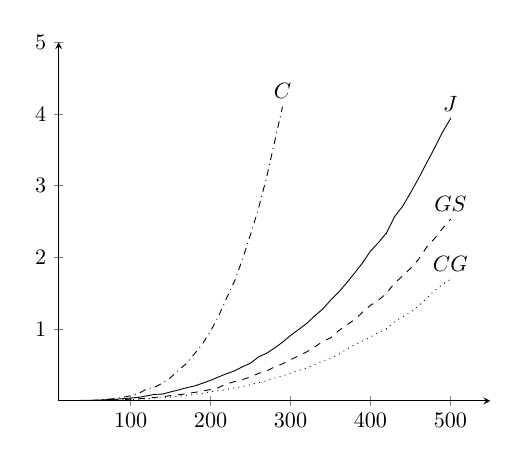
\begin{tikzpicture}[scale=0.8]
\definecolor{color0}{RGB}{0,0,0}
\begin{axis}[axis lines=middle, xmin=10, xmax=550, ymin=0.000171516, ymax=5]
\addplot[color0,  forget plot]
table{%
10 0.000171516
10.000000 0.000172
20 0.00086634
20.000000 0.000866
30 0.00327906
30.000000 0.003279
40 0.00647366
40.000000 0.006474
50 0.00667325
50.000000 0.006673
60 0.00972296
60.000000 0.009723
70 0.016745
70.000000 0.016745
80 0.0211053
80.000000 0.021105
90 0.0300734
90.000000 0.030073
100 0.0391278
100.000000 0.039128
110 0.049268
110.000000 0.049268
120 0.069232
120.000000 0.069232
130 0.089796
130.000000 0.089796
140 0.094726
140.000000 0.094726
150 0.12448
150.000000 0.124480
160 0.151938
160.000000 0.151938
170 0.183265
170.000000 0.183265
180 0.207649
180.000000 0.207649
190 0.245816
190.000000 0.245816
200 0.286124
200.000000 0.286124
210 0.333215
210.000000 0.333215
220 0.37788
220.000000 0.377880
230 0.418518
230.000000 0.418518
240 0.475069
240.000000 0.475069
250 0.525086
250.000000 0.525086
260 0.612617
260.000000 0.612617
270 0.66374
270.000000 0.663740
280 0.735477
280.000000 0.735477
290 0.817476
290.000000 0.817476
300 0.910843
300.000000 0.910843
310 0.993726
310.000000 0.993726
320 1.07653
320.000000 1.076535
330 1.18242
330.000000 1.182422
340 1.27652
340.000000 1.276515
350 1.40076
350.000000 1.400757
360 1.5122
360.000000 1.512197
370 1.64106
370.000000 1.641058
380 1.77851
380.000000 1.778514
390 1.92293
390.000000 1.922930
400 2.08742
400.000000 2.087421
410 2.2066
410.000000 2.206601
420 2.34093
420.000000 2.340928
430 2.56365
430.000000 2.563652
440 2.70883
440.000000 2.708828
450 2.89616
450.000000 2.896160
460 3.09887
460.000000 3.098874
470 3.31138
470.000000 3.311378
480 3.5203
480.000000 3.520301
490 3.74301
490.000000 3.743013
500 3.93103
500.000000 3.931026
} node[above] {$J$};
\addplot[color0, dashed, forget plot]
table{%
10 7.9231e-05
10.000000 0.000079
20 0.000481631
20.000000 0.000482
30 0.00194831
30.000000 0.001948
40 0.00417876
40.000000 0.004179
50 0.00370848
50.000000 0.003708
60 0.00614255
60.000000 0.006143
70 0.0096309
70.000000 0.009631
80 0.0126238
80.000000 0.012624
90 0.0185437
90.000000 0.018544
100 0.0235946
100.000000 0.023595
110 0.0292887
110.000000 0.029289
120 0.0379328
120.000000 0.037933
130 0.0478929
130.000000 0.047893
140 0.0567718
140.000000 0.056772
150 0.0731318
150.000000 0.073132
160 0.0838855
160.000000 0.083885
170 0.100656
170.000000 0.100656
180 0.117748
180.000000 0.117748
190 0.135347
190.000000 0.135347
200 0.157979
200.000000 0.157979
210 0.185532
210.000000 0.185532
220 0.23412
220.000000 0.234120
230 0.269388
230.000000 0.269388
240 0.296042
240.000000 0.296042
250 0.335042
250.000000 0.335042
260 0.382121
260.000000 0.382121
270 0.415055
270.000000 0.415055
280 0.473213
280.000000 0.473213
290 0.515603
290.000000 0.515603
300 0.573986
300.000000 0.573986
310 0.626939
310.000000 0.626939
320 0.681497
320.000000 0.681497
330 0.74919
330.000000 0.749190
340 0.826751
340.000000 0.826751
350 0.877331
350.000000 0.877331
360 0.975664
360.000000 0.975664
370 1.05619
370.000000 1.056190
380 1.12954
380.000000 1.129538
390 1.23362
390.000000 1.233619
400 1.33133
400.000000 1.331328
410 1.40313
410.000000 1.403128
420 1.49946
420.000000 1.499464
430 1.63992
430.000000 1.639923
440 1.73809
440.000000 1.738087
450 1.84559
450.000000 1.845589
460 1.97157
460.000000 1.971566
470 2.13758
470.000000 2.137579
480 2.26021
480.000000 2.260206
490 2.40171
490.000000 2.401708
500 2.52554
500.000000 2.525536
} node[above] {$GS$};
\addplot[color0, dotted, forget plot]
table{%
10 0.000121239
10.000000 0.000121
20 0.000604065
20.000000 0.000604
30 0.00164634
30.000000 0.001646
40 0.00283509
40.000000 0.002835
50 0.00277102
50.000000 0.002771
60 0.00467427
60.000000 0.004674
70 0.00733977
70.000000 0.007340
80 0.00981754
80.000000 0.009818
90 0.0141642
90.000000 0.014164
100 0.0180353
100.000000 0.018035
110 0.0220448
110.000000 0.022045
120 0.0291203
120.000000 0.029120
130 0.036587
130.000000 0.036587
140 0.0434833
140.000000 0.043483
150 0.052954
150.000000 0.052954
160 0.0654166
160.000000 0.065417
170 0.0764859
170.000000 0.076486
180 0.0894879
180.000000 0.089488
190 0.102215
190.000000 0.102215
200 0.128915
200.000000 0.128915
210 0.139589
210.000000 0.139589
220 0.157458
220.000000 0.157458
230 0.179333
230.000000 0.179333
240 0.199423
240.000000 0.199423
250 0.225927
250.000000 0.225927
260 0.253787
260.000000 0.253787
270 0.280379
270.000000 0.280379
280 0.317131
280.000000 0.317131
290 0.345662
290.000000 0.345662
300 0.386103
300.000000 0.386103
310 0.422678
310.000000 0.422678
320 0.4579
320.000000 0.457900
330 0.504794
330.000000 0.504794
340 0.553466
340.000000 0.553466
350 0.590098
350.000000 0.590098
360 0.647777
360.000000 0.647777
370 0.718308
370.000000 0.718308
380 0.781497
380.000000 0.781497
390 0.832744
390.000000 0.832744
400 0.888307
400.000000 0.888307
410 0.953204
410.000000 0.953204
420 1.00422
420.000000 1.004219
430 1.10199
430.000000 1.101993
440 1.16883
440.000000 1.168831
450 1.23442
450.000000 1.234425
460 1.32542
460.000000 1.325421
470 1.42446
470.000000 1.424458
480 1.53705
480.000000 1.537053
490 1.61991
490.000000 1.619915
500 1.69394
500.000000 1.693940
} node[above] {$CG$};
\addplot[color0, dashdotted, forget plot]
table{%
10 9.9297e-05
10.000000 0.000099
20 0.000700153
20.000000 0.000700
30 0.00241376
30.000000 0.002414
40 0.00452465
40.000000 0.004525
50 0.00638056
50.000000 0.006381
60 0.0127957
60.000000 0.012796
70 0.0213059
70.000000 0.021306
80 0.0320726
80.000000 0.032073
90 0.0499284
90.000000 0.049928
100 0.0718767
100.000000 0.071877
110 0.102187
110.000000 0.102187
120 0.164281
120.000000 0.164281
130 0.188823
130.000000 0.188823
140 0.249047
140.000000 0.249047
150 0.323534
150.000000 0.323534
160 0.429071
160.000000 0.429071
170 0.521841
170.000000 0.521841
180 0.657483
180.000000 0.657483
190 0.795538
190.000000 0.795538
200 0.971675
200.000000 0.971675
210 1.18065
210.000000 1.180646
220 1.43207
220.000000 1.432070
230 1.66826
230.000000 1.668258
240 1.9756
240.000000 1.975603
250 2.31886
250.000000 2.318862
260 2.68266
260.000000 2.682664
270 3.11233
270.000000 3.112333
280 3.6044
280.000000 3.604404
290 4.10074
290.000000 4.100741
} node[above] {$C$};
\end{axis}
\end{tikzpicture}

  \caption{Plots of the different time requirements for solvign the linear
  systems.}
  \label{fig:times}
\end{figure}

\subsubsection{Possitive Definite}%
\label{ssub:possitive_definite}

All of these algorithms require a positive definite matrix. This is required to
guarantee that there is a unique solution to the system. This can be considered
to ensure that there is a minimum in some $N$ dimensional space, instead of a
saddle, or maximum. Only with a minimum can we minimize our residual and use
gradient descent to find our equilibrium solution.

\subsubsection{Symmetric}%
\label{ssub:symmetric}

Most of these algorithms, with the exception of the Gauss-Seidel method,
require the matrix to be symmetric. This requirement is mostly for
computational efficiency and simplicity of the algorithm. There are some
methods that can be adapted to function for nonsymmetric matrices, but those
become significantly more complex. For our implementation we will be restricted
to the Gauss-Seidel method, as the matricies in the linear systems are not
symmetric. For better preformance, it is recommended to utilize the Generalized
Minimum Residual method, as this can handle non-symmetric matricies and is
significantly faster than Gauss-Seidel method.


\end{document}
